\section{Implementation}

The proposed mobile robot will be connected as shown in Figure~\ref{fig:Fig51} with the actual set up (as of the moment) and the exhaust fan shown in Figure~\ref{fig:Fig52}.

\begin{figure}
	\centering
	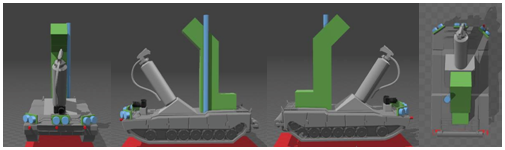
\includegraphics[width=\columnwidth]{Fig51}
	\caption{Target Mobile Robot Design}
	\label{fig:Fig51}
\end{figure}

\begin{figure}
	\centering
	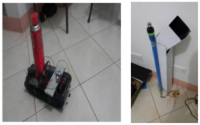
\includegraphics[width=\columnwidth]{Fig52}
	\caption{Current Mobile Robot Design}
	\label{fig:Fig52}
\end{figure}

The implementation phase of the proposed system was broken into two sub phases, the individual tests where each component of the proposed mobile robot are put into rigorous testing to their maximum capacity without breaking down, and the actual testing where everything is assembled together and the actual performance of the system can be tested. The researchers are currently in the individual tests interfacing the two Arduino UNO boards.
	The proposed algorithm for the system will be composed of two parts, the Room Handling Algorithm, and the Navigation Algorithm. The flowchart on the program flow is shown in Figures~\ref{fig:Fig53} and ~\ref{fig:Fig54} respectively.

\begin{figure}[!tb]
	\centering
	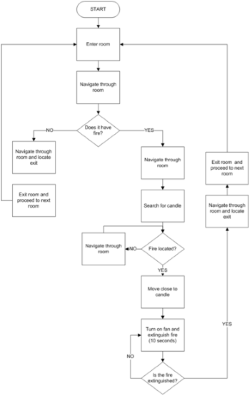
\includegraphics[width=\columnwidth]{Fig53}
	\caption{Room Handling Algorithm}
	\label{fig:Fig53}
\end{figure}

\begin{figure}
	\centering
	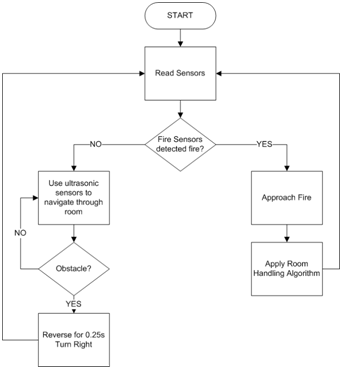
\includegraphics[width=\columnwidth]{Fig54}
	\caption{Navigation Algorithm}
	\label{fig:Fig54}
\end{figure}

\section{Evaluation}



\section{Summary}

